Here is our understanding of the efficient use of a processor so far: first, the CPU can do multiple operations at once, such as add and multiply at the same time. Not taking advantage of this capability is like leaving free computing power on the table. Second, the factor that limits our ability to maximize efficiency is how fast we can produce the data to feed into these operations. Specifically, we are constrained by the data dependencies: if one operation computed the value that the next operation uses as an input, the two operations must be executed sequentially. The workaround to this dependency is pipelining: when executing loops or long sequences of code, the processor will interleave separate computations such as loop iterations, as long as they have at least some operations that can be executed independently. 

However, pipelining has an important precondition as well. Pipelining plans ahead: in order to interleave code from several loop iterations, we must know what code will be executed. Compare this with what we learned in the last section: in order to execute instructions in parallel, we must know in advance what the input values are. Now, in order to run the instructions through the pipeline, we must know what the instructions are. Why wouldn't we know? Because the code we run often depends on the data we have: every time we encounter the if(condition) statement, we will execute either the true branch or the false branch, but we won't know which until we evaluate the condition. Just like data dependency was the bane of instruction-level parallelism, the conditional execution, or branches, are the bane of pipelining.

With pipelining disrupted, we can expect a significant reduction in the efficiency of our program. It should be very easy to modify our earlier benchmark to observe this deleterious effect of conditionals. For example, instead of writing:

\begin{lstlisting}[style=styleCXX]
a1 += p1[i] + p2[i];
\end{lstlisting}

We could write:

\begin{lstlisting}[style=styleCXX]
a1 += (p1[i]>p2[i]) ? p1[i] : p2[i];
\end{lstlisting}

Now we have reintroduced the data dependency as a code dependency:

\hspace*{\fill} \\ %插入空行
\begin{center}
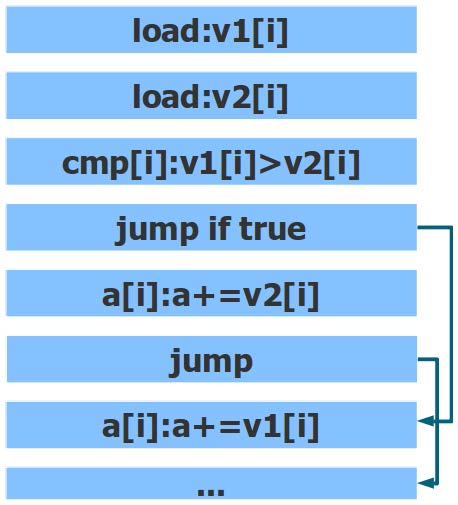
\includegraphics[width=0.9\textwidth]{content/1/chapter3/images/18.jpg}\\
Figure 3.18 – Effect of a branch instruction on the pipeline
\end{center}

There is no obvious way to convert this code into a linear stream of instructions to execute, and the conditional jump cannot be avoided.

The reality is somewhat more complex: a benchmark such as we have just suggested may or may not show significant degradation in performance. The reason is that many processors have some sort of conditional move or even conditional add instructions, and the compiler may decide to use them. If this happens, our code becomes entirely sequential with no jumps or branches and can be pipelined perfectly:

\hspace*{\fill} \\ %插入空行
\begin{center}
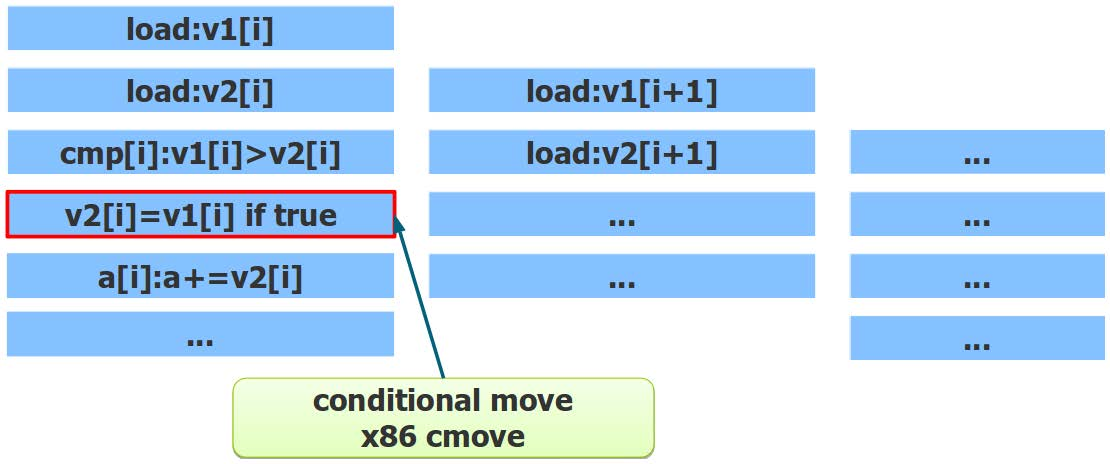
\includegraphics[width=0.9\textwidth]{content/1/chapter3/images/19.jpg}\\
Figure 3.19 – Conditional code pipelined with cmove
\end{center}

The x86 CPUs have a conditional move instruction, cmove (although not all compilers will use it to implement the ?: operator in the previous figure). The processors with AVX or AVX2 instruction sets have a powerful set of masked addition and multiplication instructions that can be used to implement some conditional code as well. That is why, when benchmarking and optimizing the code with branches, it is very important to examine the generated object code and confirm that the code indeed contains branches and that they are indeed affecting the performance. There are also profiler tools that can be used for this purpose, and we will see one such tool in a moment.

While branches and conditionals happen everywhere in most real-life programs, they can disappear when the program is reduced to just a few lines for a benchmark. One reason is that that the compiler may decide to use one of the conditional instructions we have mentioned earlier. Another reason that is common in poorly constructed benchmarks is that the compiler may be able to figure out, at compile-time, what the condition evaluates to. For example, most compilers will completely optimize away any code like if (true) or if (false): there is no trace of this statement in the generated code, and any code that is never going to be executed is also eliminated. To observe the deleterious effect of the branches on the loop pipelining, we have to construct a test where the compiler cannot predict the outcome of the condition check. In your real-life benchmarks, you may have a data set extracted from your real program. For this next demonstration, we will use random values:

\begin{lstlisting}[style=styleCXX]
\\02_branch.C

std::vector<unsigned long> v1(N), v2(N);
std::vector<int> c1(N);
for (size_t i = 0; i < N; ++i) {
	v1[i] = rand();
	v2[i] = rand();
	c1[i] = rand() & 1;
}
unsigned long* p1 = v1.data();
unsigned long* p2 = v2.data();
int* b1 = c1.data();
for (auto _ : state) {
	unsigned long a1 = 0, a2 = 0;
	for (size_t i = 0; i < N; ++i) {
		if (b1[i]) {
			a1 += p1[i];
		} else {
			a1 *= p2[i];
		}
	}
	benchmark::DoNotOptimize(a1);
	benchmark::DoNotOptimize(a2);
	benchmark::ClobberMemory();
}
\end{lstlisting}

Again, we have two input vectors v1 and v2, plus a control vector c1 that has random values of zero and one (avoid using vector<bool> here, it is not an array of bytes but a packed array of bits, so accessing it is considerably more expensive, and we are not interested in benchmarking bit manipulation instructions at this time). The compiler cannot predict whether the next random number is odd or even, thus, no optimizations are possible. Also, we have examined the generated machine code and confirmed that our compiler (Clang-11 on x86) implements this loop using a simple conditional jump. To have a baseline, we will compare the performance of this loop with one that does unconditional addition and multiplication on each iteration: a1 += p1[i]*p2[i]. This simpler loop does both an addition and a multiplication on each iteration; however, thanks to the pipelining, we get the addition free: it is executed simultaneously with the multiplication from the next iteration. The conditional branch, on the other hand, is anything but free:

\hspace*{\fill} \\ %插入空行
\begin{center}
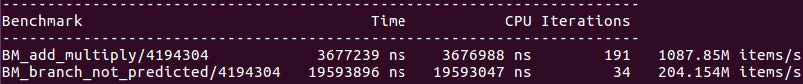
\includegraphics[width=0.9\textwidth]{content/1/chapter3/images/20.jpg}\\
Figure 3.20
\end{center}

As you can see, the conditional code is about five times slower than the sequential one. This confirms our prediction that when the next instruction depends on the result of the previous one, the code cannot be effectively pipelined.


\subsubsubsection{3.5.1\hspace{0.2cm}Branch prediction}

However, an astute reader may point out that the picture we have just described cannot possibly be complete, or even true: let us go back, for a moment, to the apparently linear code such as the loop we have used extensively in the last section:

\begin{lstlisting}[style=styleCXX]
	for (size_t i = 0; i < N; ++i) {
		a1 += v1[i] + v2[i]; // s[i] = v1[i] + v2[i]
	}
\end{lstlisting}

Here is what the body of this loop looks like from the processor's point of view:

\hspace*{\fill} \\ %插入空行
\begin{center}
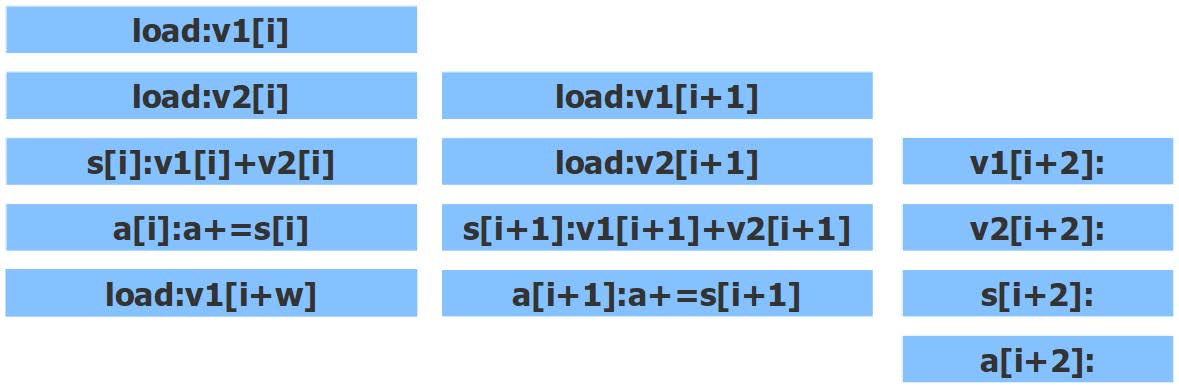
\includegraphics[width=0.9\textwidth]{content/1/chapter3/images/21.jpg}\\
Figure 3.21 – Loop executed in a pipeline of width w
\end{center}

In Figure 3.21, we have shown three interleaved iterations, but there could be even more, the total width of the pipeline is w, and ideally, w is large enough that at every cycle, the CPU is executing exactly as many instructions as it can execute simultaneously (such peak efficiency is rarely possible in practice). Note, however, that it may be impossible to access v[i+2] at the same time as we compute the sum p1[i] + p2[i]: there is no guarantee that the loop has two more iterations to go, and, if it doesn't, the element v[i+2] does not exist and accessing it results in undefined behavior. There is a hidden conditional in the previous code: at every iteration, we must check if i is less than N, and only then can we execute the instructions of the i-th iteration. 

Therefore, our comparison in Figure 3.20 is a lie: we did not compare pipelined sequential execution versus an unpredictable conditional one. Both benchmarks are, in fact, examples of conditional code, they both have branches.

The full truth is somewhere in between. To understand it, we have to learn about the antidote to the conditional execution, which poisons the pipelining and is itself the antidote to the data dependency. The way to save the pipelining in the presence of branches is to attempt to convert the conditional code to the sequential one. Such conversion could be done if we knew in advance which path the branch is going to take: we would simply eliminate the branch and proceed to the next instruction to be executed. Of course, there would be no need even to write such code if we knew in advance what the condition is. Still, consider the loop termination condition. Assuming the loop is executed many times, it is a good bet that the condition i < N evaluates to true (we would lose this bet only one out of N times).

The processor makes the same bet using the technique known as branch prediction. It analyzes the history of every branch in the code and assumes that the behavior will not change in the future. For the end of the loop condition, the processor will quickly learn that most of the time, it has to proceed to the next iteration. Therefore, the right thing to do is to pipeline the next iteration as if we are sure it's going to happen. Of course, we have to defer the actual writing of the results into memory until we evaluate the condition and confirm that the iteration does happen; the processor has a certain number of write buffers to hold such unconfirmed results in limbo before committing them to memory.

The pipeline for the loop with just an addition, therefore, does look exactly as shown in Figure 3.21. The only catch is that, when starting to execute iteration i+2 before the i-th iteration is complete, the processor is making a bet based on its prediction of whether the conditional branch will be taken or not. Such execution of the code before we know for sure that this code really exists is known as speculative execution. If the bet is won, we already have the results by the time we figure out that we needed the computation, and all is well. If the processor loses the bet, it has to discard some of the computations to avoid producing incorrect results: for example, writing into memory overwrites what was there before and cannot be undone on most hardware platforms, while computing the result and storing it in a register is entirely reversible, except for the time we wasted, of course.

We now have a more complete picture of how the pipelining really works: in order to find more instructions to execute in parallel, the processor looks at the code for the next iterations of the loop and starts to execute it simultaneously with the current iteration. If the code includes a conditional branch, which makes it impossible to know for sure which instruction will be executed, the processor makes an educated guess based on the past outcomes of checking the same condition and proceeds to execute the code speculatively. If the prediction proves to be correct, the pipelining can be as good as it was for the unconditional code. If the prediction is wrong, the processor has to discard the result of every instruction that should not have been evaluated, fetch the instructions that it previously assumed wouldn't be needed, and evaluate them instead. This event is called a pipeline flush, and it is an expensive occurrence indeed.

Now we have a better understanding of our previous benchmark in Figure 3.20: both loops have a condition for checking the end of the loop. However, it is predicted almost perfectly. The pipeline flush occurs only once at the end of the loop. The conditional benchmark also has a branch that is based on a random number: if(b1[i]) where b1[i] is true 50\% of the time, randomly. The processor is powerless to predict the outcome, and the pipeline is disrupted half the time (or worse, if we manage to confuse the CPU into actually making wrong predictions).

We should be able to verify our understanding with a direct experiment: all we need is to change the random condition to something that is always true. The only catch is that we have to do it in a way that the compiler cannot figure it out. One common way is to change the initialization of the condition vector as follows:

\begin{lstlisting}[style=styleCXX]
c1[i] = rand() >= 0;
\end{lstlisting}

The compiler doesn't know that the function rand() always returns non-negative random numbers and will not eliminate the condition. The branch predictor circuit of the CPU will quickly learn that the condition if(b1[i]) always evaluates to true and will execute the corresponding code speculatively. We can compare the performance of the well-predicted branch with that of the unpredictable one:

\hspace*{\fill} \\ %插入空行
\begin{center}
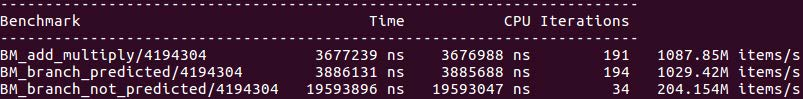
\includegraphics[width=0.9\textwidth]{content/1/chapter3/images/22.jpg}\\
Figure 3.22
\end{center}

Here we can see that the cost of the well-predicted branch is minimal and that it is much faster than exactly the same code with a branch that is predicted poorly.

\subsubsubsection{3.5.2\hspace{0.2cm}Profiling for branch mispredictions}

Now that you have seen how badly a single mispredicted branch can impact the performance of the code, you may wonder, how would you ever find such code so you can optimize it? Sure, the function containing this code will take longer than you might expect, but how do you know whether it's because of the badly predicted branches or due to some other inefficiency? By now, you should know enough to avoid making guesses about performance in general; however, speculating about the effectiveness of the branch predictor is particularly futile. Fortunately, most profilers can profile not just execution time but also various factors determining the efficiency, including the branch prediction failures.

In this chapter, we will once again use the perf profiler. As the first step, we can run this profiler to collect the overall performance metrics of the entire benchmark program:

\begin{tcblisting}{commandshell={}}
$ perf stat ./benchmark
\end{tcblisting}

Here are the perf results for the program running only the BM\_branch\_not\_predicted benchmark (other benchmarks are commented out for this test):

\hspace*{\fill} \\ %插入空行
\begin{center}
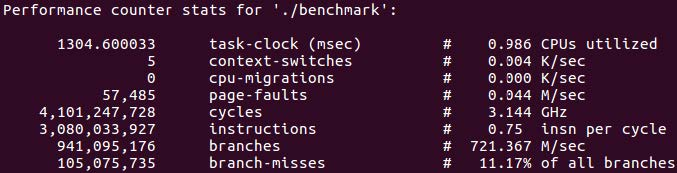
\includegraphics[width=0.9\textwidth]{content/1/chapter3/images/23.jpg}\\
Figure 3.23 – Profile of a benchmark with a poorly predicted branch
\end{center}

As you can see, 11\% of all branches were mispredicted (the last line of the report). Note that this number is cumulative for all branches, including the perfectly predictable end of the loop condition, so 11\% total is quite bad. We should compare it with our other benchmark, BM\_branch\_predicted, which is identical to this one except the condition is always true:

\hspace*{\fill} \\ %插入空行
\begin{center}
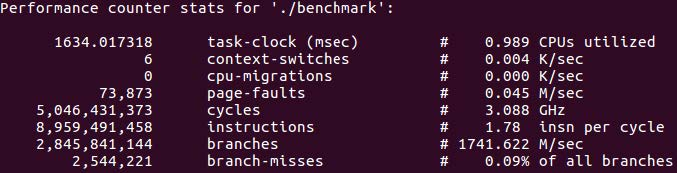
\includegraphics[width=0.9\textwidth]{content/1/chapter3/images/24.jpg}\\
Figure 3.24 – Profile of a benchmark with a well-predicted branch
\end{center}

This time, less than 0.1\% of all branches were not predicted correctly.

The overall performance report is very useful, do not ignore its potential: it can be used to highlight or dismiss some possible causes of poor performance quickly. In our case, we can immediately conclude that our program suffers from one or more mispredicted branches. Now we just need to find which one, and the profiler can help with that as well. Just like in the previous chapter, where we have used the profiler to find out where in the code does our program spends the most time, we can generate a detailed line-by-line profile of branch predictions. We just need to specify the right performance counter to the profiler:

\begin{tcblisting}{commandshell={}}
$ perf record -e branches,branch-misses ./benchmark
\end{tcblisting}

In our case, we can copy the name of the counter from the output of perf stat, because it happens to be one of the counters it measures by default, but the complete list can be obtained by running perf --list.

The profiler runs the program and collects the metrics. We can view them by generating a profile report:

\begin{tcblisting}{commandshell={}}
$ perf report
\end{tcblisting}

The report analyzer is interactive and lets us navigate to the branch mispredictions counter for each function:

\hspace*{\fill} \\ %插入空行
\begin{center}
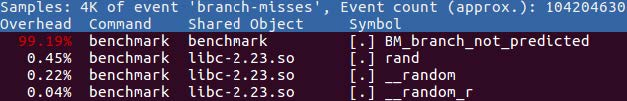
\includegraphics[width=0.9\textwidth]{content/1/chapter3/images/25.jpg}\\
Figure 3.25 – Detailed profile report for mispredicted branches
\end{center}

Over 99\% of all mispredicted branches occur in just one function. Since the function is small, finding the responsible conditional operation should not be hard. In a larger function, we would have to look at the line-by-line profile.

The branch prediction hardware of a modern processor is fairly sophisticated. For example, if a function is called from two different places and, when called from the first place, a condition usually evaluates to true, while, when called from the second place, the same condition evaluates to false, the predictor will learn that pattern and predict the branch correctly based on the origin of the function call. Similarly, the predictor can detect fairly complex patterns in the data. For example, we can initialize our random condition variables so that the values always alternate, the first one is random, but the next one is the opposite of the first one, and so on:

\begin{lstlisting}[style=styleCXX]
for (size_t i = 0; i < N; ++i) {
	if (i == 0) c1[i] = rand() >= 0;
	else c1[i] = !c1[i - 1];
}
\end{lstlisting}

The profiler confirms that the branch prediction rate for this data is excellent:

\hspace*{\fill} \\ %插入空行
\begin{center}
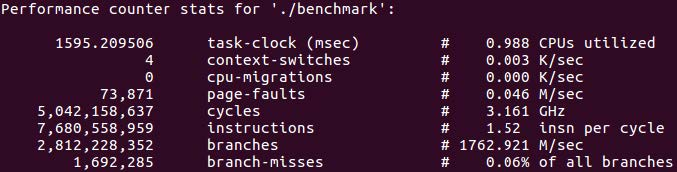
\includegraphics[width=0.9\textwidth]{content/1/chapter3/images/26.jpg}\\
Figure 3.26 – Branch prediction rate for a "true-false" pattern
\end{center}

We are almost ready to apply our knowledge of how to use the processor efficiently. But first, I must admit that we have overlooked a major potential problem. 































